\documentclass[11pt]{article}
\usepackage{listings}
\usepackage{tikz}
\usepackage{algorithm2e}
\usepackage{enumerate}
\usepackage{multicol}
\usetikzlibrary{arrows,automata,shapes}
\tikzstyle{block} = [rectangle, draw, fill=blue!20, 
    text width=5em, text centered, rounded corners, minimum height=2em]
\tikzstyle{bt} = [rectangle, draw, fill=blue!20, 
    text width=1em, text centered, rounded corners, minimum height=2em]

\newtheorem{defn}{Definition}
\newtheorem{crit}{Criterion}

\newcommand{\handout}[5]{
  \noindent
  \begin{center}
  \framebox{
    \vbox{
      \hbox to 5.78in { {\bf Software Testing, Quality Assurance and Maintenance } \hfill #2 }
      \vspace{4mm}
      \hbox to 5.78in { {\Large \hfill #5  \hfill} }
      \vspace{2mm}
      \hbox to 5.78in { {\em #3 \hfill #4} }
    }
  }
  \end{center}
  \vspace*{4mm}
}

\newcommand{\lecture}[4]{\handout{#1}{#2}{#3}{#4}{Lecture #1}}
\topmargin 0pt
\advance \topmargin by -\headheight
\advance \topmargin by -\headsep
\textheight 8.9in
\oddsidemargin 0pt
\evensidemargin \oddsidemargin
\marginparwidth 0.5in
\textwidth 6.5in

\parindent 0in
\parskip 1.5ex
%\renewcommand{\baselinestretch}{1.25}
% http://gurmeet.net/2008/09/20/latex-tips-n-tricks-for-conference-papers/
\newcommand{\squishlist}{
 \begin{list}{$\bullet$}
  { \setlength{\itemsep}{0pt}
     \setlength{\parsep}{3pt}
     \setlength{\topsep}{3pt}
     \setlength{\partopsep}{0pt}
     \setlength{\leftmargin}{1.5em}
     \setlength{\labelwidth}{1em}
     \setlength{\labelsep}{0.5em} } }
\newcommand{\squishlisttwo}{
 \begin{list}{$\bullet$}
  { \setlength{\itemsep}{0pt}
     \setlength{\parsep}{0pt}
    \setlength{\topsep}{0pt}
    \setlength{\partopsep}{0pt}
    \setlength{\leftmargin}{2em}
    \setlength{\labelwidth}{1.5em}
    \setlength{\labelsep}{0.5em} } }
\newcommand{\squishend}{
  \end{list}  }

\begin{document}

\lecture{16 --- February 9, 2015}{Winter 2015}{Patrick Lam}{version 2}

\section*{Subsumption Chart} Here are the subsumption relationships
between our graph criteria. %Assume Best-Effort Touring.

\tikzstyle{bw} = [rectangle, draw, fill=blue!20, 
    text width=12em, text centered, rounded corners, minimum height=2em]
\tikzstyle{bww} = [rectangle, draw, fill=blue!20, 
    text width=14.2em, text centered, rounded corners, minimum height=2em]

\begin{center}
\label{SC}
\begin{tikzpicture}[->,>=stealth',shorten >=1pt,auto,node distance=24mm,
                    semithick,initial text=]

  \node[bw]   (CPC)               {$\frac{\mbox{Complete Path Coverage}}{\mbox{CPC}}$};
  \node[bw]   (PPC) [below of=CPC] {$\frac{\mbox{Prime Path Coverage}}{\mbox{PPC}}$};
  \node[bw]   (ADUPC) [below left of=PPC,xshift=-40mm] {$\frac{\mbox{All-du-Paths Coverage$^*$}}{\mbox{ADUPC}}$};
  \node[bw]   (AUC) [below of=ADUPC] {$\frac{\mbox{All-Uses Coverage}}{\mbox{AUC}}$};
  \node[bw]   (ADC) [below of=AUC] {$\frac{\mbox{All-Defs Coverage}}{\mbox{ADC}}$};

  \node[bw]   (EPC) [right of=ADUPC,xshift=30mm] {$\frac{\mbox{Edge-Pair Coverage}}{\mbox{EPC}}$};
  \node[bw]   (EC) [below of=EPC] {$\frac{\mbox{Edge Coverage}}{\mbox{EC}}$};
  \node[bw]   (NC) [below of=EC] {$\frac{\mbox{Node Coverage}}{\mbox{NC}}$};

  \node[bww]   (CRTC) [right of=EPC,xshift=35mm] {$\frac{\mbox{Complete Round-Trip Coverage$^*$}}{\mbox{CRTC}}$};
  \node[bww]   (SRTC) [below of=CRTC] {$\frac{\mbox{Simple Round-Trip Coverage$^*$}}{\mbox{SRTC}}$};

  \path (CPC) edge node {} (PPC)
        (PPC) edge node {} (ADUPC)
        (ADUPC) edge node {} (AUC)
        (AUC) edge node {} (ADC)
              edge node {} (EC)
        (EPC) edge node {} (EC)
        (PPC) edge [bend left] node  {} (EC)
        (EC) edge node {} (NC)
        (PPC) edge node {} (CRTC)
        (CRTC) edge node {} (SRTC);

\end{tikzpicture}
\end{center}

\begin{itemize}
\item We know EPC subsumes EC subsumes NC from before, and clearly
CRTC subsumes SRTC. Also, CPC subsumes PPC and PPC subsumes EPC. PPC
subsumes CRTC, because simple paths include round trips.
\item In this offering, we didn't talk about ADUPC at all, and we only touched briefly on CRTC and SRTC.
\end{itemize}

Assumptions for dataflow criteria:
\begin{enumerate}
\item every use preceded by a def (guaranteed by Java)
\item every def reaches at least one use
\item for every node with multiple outgoing edges, at least 
one variable is used on each out edge, and the same variables
are used on each out edge.
\end{enumerate}

Then: 
\begin{itemize}
\item AUC subsumes ADC.
\item Each edge has at least one use, so AUC subsumes EC.
\item Finally, each {\em du}-path is also a simple path, so PPC
  subsumes ADUPC (not discussed this term, but ADUPC subsumes
  AUC). (Note that prime paths are simpler to compute than data flow
  relationships, especially in the presence of pointers.
\end{itemize}

\section*{Dataflow Graph Coverage for Source Code}

Last time, we saw how to construct graphs which summarized
a control-flow graph's structure. Let's enrich our CFGs with
definitions and uses to enable the use of our dataflow criteria.

\paragraph{Definitions.} Here are some Java statements which
correspond to definitions.

\begin{itemize}
\item {\tt x = 5}: {\tt x} occurs on the left-hand side of
an assignment statement;
\item {\tt foo(T x) \{ ... \} }: implicit definition for {\tt x}
at the start of a method;
\item {\tt bar(x)}: during a call to {\tt bar}, {\tt x} might
be defined if {\tt x} is a C++ reference parameter.
\item (subsumed by others): {\tt x} is an input to the program.
\end{itemize}

{\sf Examples:} \\[2em]
% void bar(int& c) { c = 5; } bar(x)
% x = System.in.readLines(); argv is a formal parameter

\paragraph{Uses.} The book lists a number of cases of uses, but
it boils down to ``{\tt x} occurs in an expression that the program
evaluates.'' Examples: RHS of an assignment, or as part of a method
parameter, or in a conditional.

\paragraph{Complications.} 
As I said before, the situation in real-life is more complicated:
we've assumed that {\tt x} is a local variable with scalar type.
\begin{itemize}
\item What if {\tt x} is a static field, an array, an object, or an
instance field?
\item How do we deal with aliasing? 
\end{itemize}

\newpage
One answer is to be conservative and note that we've said that a
definition $d$ reaches a use $u$ if it is possible that the address
defined at $d$ refers to the same address used at $u$. For 
instance:

{\scriptsize
\begin{lstlisting}
    class C { int f; }
    void foo(C q) { use(q.f); }

    x = new C(); x.f = 5;
    y = new C(); y.f = 2;

    foo(x);
    foo(y);
\end{lstlisting}
}
Our definition says that both definitions reach the use.

\paragraph{Exercise.} Consider the following graph:
\begin{itemize}
\item $N = \{0, 1, 2, 3, 4, 5, 6, 7\}$
\item $N_0 = \{ 0 \}$
\item $N_f = \{ 7 \}$
\item $E = \{ (0, 1), (1, 2), (1, 7), (2, 3), (2, 4), (3, 2), (4, 5), (4, 6), (5, 6), (6, 1) \}$
\item test paths: \begin{itemize}
\item $t_1 = [0,1,7]$
\item $t_2 = [0,1,2,4,6,1,7]$
\item $t_3 = [0,1,2,4,5,6,1,7]$
\item $t_4 = [0,1,2,3,2,4,6,1,7]$
\end{itemize}
  \item def(0) = def(3) = use(5) = use(7) = \{ $x$ \}
\end{itemize}

\begin{enumerate}[(a)]
\item Draw the graph.
\item List all {\it du}-paths with respect to $x$. Include
  all {\it du}-paths, even those that are subpaths of others.
% dropped the concept of du-tours, so no:
%\item For each test path $t$, determine which {\it du}-paths
  %  path $t$ du-tours.
\item List a minimal test set (using the given paths)
  satisfying all-defs coverage with respect to $x$.
\item List a minimal test set (using the given paths)
  satisfying all-uses coverage with respect to $x$.
\end{enumerate}

\paragraph{Compiler tidbit.} In a compiler, we use 
intermediate representations to simplify expressions, 
including definitions and uses. {\sf For instance, 
we would simplify:}

\begin{verbatim}
x  = foo(y + 1, z * 2)
\end{verbatim}

\paragraph{Basic blocks and defs/uses.} Basic
blocks can rule out some definitions and uses as irrelevant.

\begin{itemize} 
\item Defs: consider the last definition of a variable in a basic
block. (If we're not sure whether {\tt x} and {\tt y} are aliased,
leave both of them.)
\item Uses: consider only uses that aren't dominated by a
definition of the same variable in the same basic block, e.g.
{\tt y = 5; use(y)} is not interesting.
\end{itemize}

\section*{Graph Coverage for Design Elements}
We next move beyond single methods to ``design elements'', which
include multiple methods, classes, modules, packages, etc. Usually
people refer to such testing as ``integration testing''.

\vspace*{-1em}
\subsection*{Structural Graph Coverage.} We want to create graphs
that represent relationships---\emph{couplings}---between design elements.
\vspace*{-1em}

\paragraph{Call Graphs.} Perhaps the most common interprocedural
graph is the \emph{call graph}.
\squishlist
\item design elements, or nodes,
are methods (or larger program subsystems)
\item couplings, or edges, are method calls.
\squishend

Consider the following example.
\vspace*{-1em}
\begin{center}
\label{CFG}
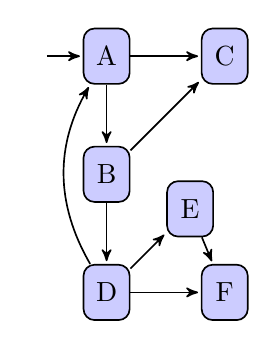
\begin{tikzpicture}[->,>=stealth',shorten >=1pt,auto,node distance=1.5cm,
                    semithick,initial text=]

  \node[initial,bt]   (A)                     {A};
  \node[bt]           (B) [below of=A] {B};
  \node[bt]           (C) [right of=A] {C};
  \node[bt]           (D) [below of=B] {D};
  \node[bt]           (E) [above right of=D] {E};
  \node[bt]           (F) [right of=D] {F};

  \path (A) edge node {} (B)
            edge node {} (C)
        (B) edge node {} (C)
            edge node {} (D)
        (D) edge node {} (E)
            edge node {} (F)
            edge [bend left] node {} (A)
        (E) edge node {} (F);
\end{tikzpicture}
\end{center}
\vspace*{-1em}

\begin{itemize}
\item For method coverage, must call each method. 
\item For edge coverage, must visit each edge; in this particular
  case, must get to both A and C from both of their respective
  callees.
\end{itemize}
\vspace*{-1em}
Like any other type of testing, call graph-based testing may require 
test harnesses. Imagine, for instance, a library that implements a
stack; it exposes {\tt push} and {\tt pop} methods, but needs a test
driver to exercise these methods.

\vspace*{-1em}
\section*{Data Flow Graph Coverage for Design Elements}
\vspace*{-1em}

The structural coverage criteria for design elements were not very
satisfying: basically we only had call graphs. Let's instead
talk about data-bound relationships between design elements.

\squishlist
\item \emph{caller:} unit that invokes the callee;
\item \emph{actual parameter:} value passed to the callee by the caller; and
\item \emph{formal parameter:} placeholder for the incoming variable.
\squishend

\vspace*{-1em}
\paragraph{Illustration.} ~\\[-1em]

\begin{multicols}{2}{
caller:
\verb+foo(actual1, actual2);+
  }
  ~\\
{
callee:\vspace*{-1em}
\verb+void foo(int formal1, int formal2) { }+
}
\end{multicols}

\end{document}

